\section{DDS module}\label{sec:dds-module}

In this section, the DDS (Direct Digital Synthesiser) modules implemented in the project will be discussed.

Below follows the implementation used in the final version of the project:
\begin{lstlisting}[caption=Pseudo-code for final DDS implementation]
	* Parameter definitions are used for
		- NBITS_PHASE: # of bits of phase
		- NBITS_PHASE_FRAC: # of bits of fractionary part of phase
		- NSAMPLES_LUT: # of samples used in the LUT (Lookup Table)
		- HEXVAL: string containing the path for the values to be inserted in the LUT
	* Values are uploaded from the file to the LUT using $readmemh()
	* With posedge clock, if reset is not active:
		- if enableclk input is active, then phase must be updated
		- outsine output is updated in accordance with the latest value of phase
\end{lstlisting}

Besides this, a second DDS implementation was developed with the purpose of reducing the final circuit size. To achieve this, a module taking advantage of the periodicity properties of the wave, shown in \autoref{fig:sine-matlab}, was implemented.

\begin{figure}[!h]
\centering
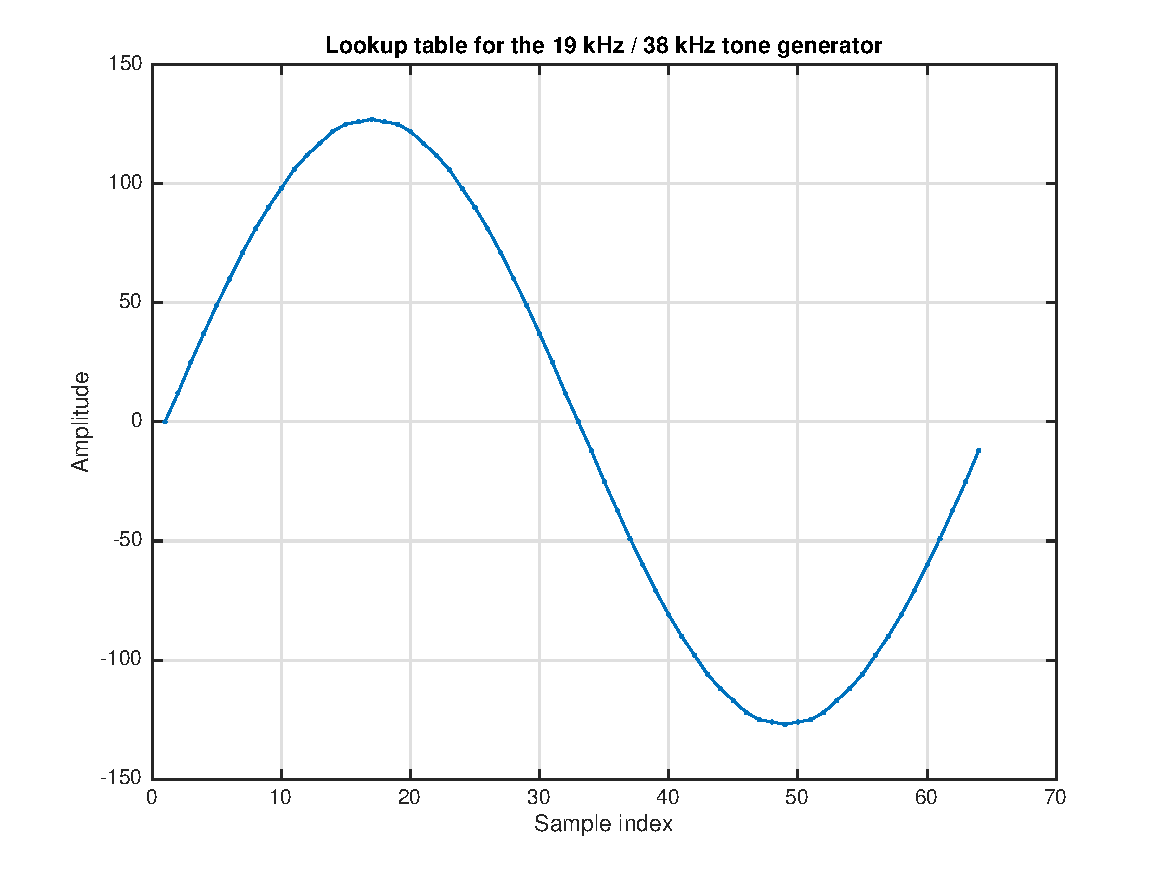
\includegraphics[width=0.7\textwidth]{sine-matlab.pdf}
\caption{Sine wave waveform and LUT values}\label{fig:sine-matlab}
\end{figure}

%% Não esquecer de falar sobre os erros corrigidos na bench do prof 8)

Because the number of samples of the LUT is a power of two, it is possible to infer the complete signal by only storing a fraction of the signal. This allowed for a reduction of the size of the LUT by 75\%. Upon further testing, it was verified that this implementation provides for area optimisations. Among others, the number of block RAM/FIFO was reduced from 1 to 0 (as seen in \autoref{table:device-utilisation}).

The module was implemented as follows:

\begin{lstlisting}[caption=Pseudo-code for an optimised implementation of the DDS]
	* Parameter definitions are used for
		- NBITS_PHASE: # of bits of phase
		- NBITS_PHASE_FRAC: # of bits of fractionary part of phase
		- NBITS_OUTPUT: # of bits in the output
		- NSAMPLES_LUT: # of samples used in the LUT (Lookup Table)
		- HEXVAL: string containing the path for the values to be inserted in the LUT
	* Values are uploaded from the file to the LUT using $readmemh()
	* sineLUT_i variable is assigned to translate the previously used phase logic to a logic that supports a smaller LUT
	
	* With posedge clock, if reset is not active:
		- if enableclk input is active, then phase must be updated
		- if value of phase equals NSAMPLES_LUT/4, sine output equals to the maximum representation value
		- if value of phase equals 3*NSAMPLES_LUT/4, sine output equals to the minimum representation value
		- else, if phase[NBITS_PHASE-1] (the MSB for phase representation is enabled), then values should be output from the LUT as negative
		- else, values should be output as is from the LUT
\end{lstlisting}













